\documentclass[a4paper, 11pt]{article}
\usepackage{geometry}
\geometry{letterpaper, margin=1in}
\usepackage{amsmath}
\usepackage{amssymb}  
\usepackage{amsthm}
\usepackage{ulem} 
\usepackage{graphicx}
\graphicspath{ {images/} }

\begin{document}
%Header-Make sure you update this information!!!!
\noindent
\large\textbf{Complex Analysis - MTH 483} \hfill \textbf{John Waczak} \\
\normalsize Day 3 \hfill  Date: \today \\

\section*{A little bit about topology}
First a couple of standard notations... \\

\textbf{Open Disk} centered at $a\in\mathbb{C}$ with radius $r>0$ is denoted by:
	\begin{equation}
		D_r(a) = \{z\in\mathbb{C}| |z-a|<r\}
	\end{equation}
	\begin{figure}[!hbt]
		\centering
		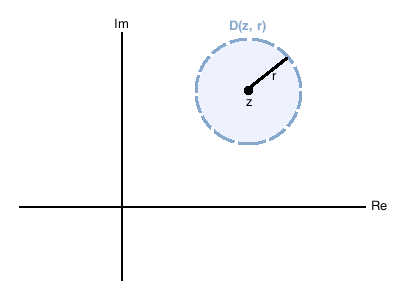
\includegraphics[scale=0.75]{disk}
	\end{figure}

The \textbf{closed disk} is given by $\overline{D}_r(a) = \{z\in\mathbb{C}| |z-a|\leq r\}$. I.e. includes the boundary. \\

A subset U of $\mathbb{C}$ is \textbf{open} if, $\forall$ $z_0 \in U$ there exists $\epsilon > 0$ for which:
	\begin{equation*}
		D_\epsilon(z_0) \subseteq U
	\end{equation*}

In other words, every point of U is contained in an open disk entirely contained in U. \\

Examples: $\emptyset$, $\mathbb{C}$, $D_r(a)$, ... are all open sets. \\

Let U be an open subset of $\mathbb{C}$. We say that U is \textbf{connected} if $\nexists$ open subsets $A, B \subset U$ such that: 
	\begin{align}
		U &= A \cup B \\ 
		A &\neq \emptyset, \quad B \neq \emptyset \\ 
		A &\cap B = \emptyset	
	\end{align}

Ex: $U = \mathbb{C}\setminus\{z=x+iy:y=0\}$ is \textit{not connected}.



\section*{Derivatives}

Let $U\subset \mathbb{C}$ and let $z_0 \in U$ and let $G:U\setminus\{z_0\}\rightarrow \mathbb{C}$ be a function. We say that:
	\begin{equation}
		L  = \lim_{z\rightarrow z_0}G(z)
	\end{equation}
exists if, $\forall$ $\epsilon>0$, $\exists$ $\delta>0$ (possibly depending on $\epsilon$) such that, if:
	\begin{equation}
		|z-z_0|< \delta \rightarrow |G(z)-L|< \epsilon 
	\end{equation}
	
\textit{Remark:} The limit concerns values of $G(z)$ as z \textit{approaches} $z_0$ from all directions... a much stronger condition than normal limit. \\

\noindent A \textbf{Region} is an \textit{open, connected, nonempty} subset of $\mathbb{C}$. \\

Let $f:\Omega \rightarrow mathbb{C}$ be a function where $\Omega$ is a region in $\mathbb{C}$. Let $z_0\in\Omega$. We say f is \textbf{Differentiable} at $z_0$ if:
	\begin{equation}
		\lim_{z\rightarrow z_0} \frac{f(z)-f(z_0)}{z-z_0} \quad \text{exists}
	\end{equation}
	
\noindent If it does exist, we call this limit $f'(z_0)$. If f is differentiable $\forall z_0 \in \Omega$ then we say f is \textbf{Holomorphic} on $\Omega$. 


\noindent If $f:\mathbb{C} \rightarrow \mathbb{C}$ is holomorphic, then we say f is \textbf{entire}. \\ \\ \\

\noindent Example: Show $f(z) = z^2$ is entire. Moreover,  $f'(z) = 2z$. \\
Let $\epsilon > 0$, and let $z_0 \in \mathbb{C}$. Then, 
	\begin{align*}
		\Big|\frac{f(z)-f(z_0)}{z-z_0}-2z_0\Big| &= \Big|\frac{z^2-z_0^2}{z-z_0}-2z_0\Big| \\ 
			&= \Big| \frac{(z-z_0)(z+z_0)}{(z-z_0)} - 2z_0\Big| \\ 
			&= |z+z_0-2z_0| = |z-z_0|
	\end{align*}
Thus if we select $\delta = \epsilon$, then $|z-z_0| < \delta \rightarrow \Big|\frac{f(z)-f(z_0)}{z-z_0}-2z_0\Big|<\epsilon$. \\ \\ \\

\noindent It is \textit{MUCH} easier to not be complex differentiable than real differentiable. Example: $f(z) = \overline{z}$ i.e. $f(x+iy) = x-iy$. 
	\begin{align*}
		\text{recall definition: } \quad& A = \lim_{h\rightarrow 0}\frac{f(z_0+h)-f(z_0)}{h} \\ 
		\text{let } z_0 &= x_0 + iy_0 \\ 
		\text{thus } A &= \lim_{h\rightarrow 0}\frac{x_0-iy_0+h-x_0+iy_0}{h} \\ 
			&= \frac{h}{h} = 1
	\end{align*}
Now let's take the limit vertically since we must be able to approach from \textit{all} directions.
	\begin{align*}
		B &= \lim_{t\rightarrow 0}\frac{f(z_0+it)-f(z_0)}{it} \\ 
			&= \lim_{t\rightarrow 0}\frac{x_0-iy_0-it-x_0+iy_0}{it} \\
			&= \lim_{t\rightarrow 0}\frac{-it}{it} = -1
	\end{align*}
Thus since $A\neq B$, $f$ is not differentiable $\forall z_0$ and therefore f is \textit{not} holomorphic. \\

\noindent Examples of holomorphic functions:
	\begin{enumerate}
		\item Polynomials are entire
		\item Rational functions $\frac{p(z)}{q(z)}$ where $q(z)\neq 0$
		\item Functions defined by convergent Power series e.g. $\sum_{n=0}^\infty \frac{z^n}{n!} = e^z$
	\end{enumerate}
\end{document}
























